\documentclass[twoside]{book}

% Packages required by doxygen
\usepackage{fixltx2e}
\usepackage{calc}
\usepackage{doxygen}
\usepackage[export]{adjustbox} % also loads graphicx
\usepackage{graphicx}
\usepackage[utf8]{inputenc}
\usepackage{makeidx}
\usepackage{multicol}
\usepackage{multirow}
\PassOptionsToPackage{warn}{textcomp}
\usepackage{textcomp}
\usepackage[nointegrals]{wasysym}
\usepackage[table]{xcolor}

% Font selection
\usepackage[T1]{fontenc}
\usepackage[scaled=.90]{helvet}
\usepackage{courier}
\usepackage{amssymb}
\usepackage{sectsty}
\renewcommand{\familydefault}{\sfdefault}
\allsectionsfont{%
  \fontseries{bc}\selectfont%
  \color{darkgray}%
}
\renewcommand{\DoxyLabelFont}{%
  \fontseries{bc}\selectfont%
  \color{darkgray}%
}
\newcommand{\+}{\discretionary{\mbox{\scriptsize$\hookleftarrow$}}{}{}}

% Page & text layout
\usepackage{geometry}
\geometry{%
  a4paper,%
  top=2.5cm,%
  bottom=2.5cm,%
  left=2.5cm,%
  right=2.5cm%
}
\tolerance=750
\hfuzz=15pt
\hbadness=750
\setlength{\emergencystretch}{15pt}
\setlength{\parindent}{0cm}
\setlength{\parskip}{3ex plus 2ex minus 2ex}
\makeatletter
\renewcommand{\paragraph}{%
  \@startsection{paragraph}{4}{0ex}{-1.0ex}{1.0ex}{%
    \normalfont\normalsize\bfseries\SS@parafont%
  }%
}
\renewcommand{\subparagraph}{%
  \@startsection{subparagraph}{5}{0ex}{-1.0ex}{1.0ex}{%
    \normalfont\normalsize\bfseries\SS@subparafont%
  }%
}
\makeatother

% Headers & footers
\usepackage{fancyhdr}
\pagestyle{fancyplain}
\fancyhead[LE]{\fancyplain{}{\bfseries\thepage}}
\fancyhead[CE]{\fancyplain{}{}}
\fancyhead[RE]{\fancyplain{}{\bfseries\leftmark}}
\fancyhead[LO]{\fancyplain{}{\bfseries\rightmark}}
\fancyhead[CO]{\fancyplain{}{}}
\fancyhead[RO]{\fancyplain{}{\bfseries\thepage}}
\fancyfoot[LE]{\fancyplain{}{}}
\fancyfoot[CE]{\fancyplain{}{}}
\fancyfoot[RE]{\fancyplain{}{\bfseries\scriptsize Generated by Doxygen }}
\fancyfoot[LO]{\fancyplain{}{\bfseries\scriptsize Generated by Doxygen }}
\fancyfoot[CO]{\fancyplain{}{}}
\fancyfoot[RO]{\fancyplain{}{}}
\renewcommand{\footrulewidth}{0.4pt}
\renewcommand{\chaptermark}[1]{%
  \markboth{#1}{}%
}
\renewcommand{\sectionmark}[1]{%
  \markright{\thesection\ #1}%
}

% Indices & bibliography
\usepackage{natbib}
\usepackage[titles]{tocloft}
\setcounter{tocdepth}{3}
\setcounter{secnumdepth}{5}
\makeindex

% Hyperlinks (required, but should be loaded last)
\usepackage{ifpdf}
\ifpdf
  \usepackage[pdftex,pagebackref=true]{hyperref}
\else
  \usepackage[ps2pdf,pagebackref=true]{hyperref}
\fi
\hypersetup{%
  colorlinks=true,%
  linkcolor=blue,%
  citecolor=blue,%
  unicode%
}

% Custom commands
\newcommand{\clearemptydoublepage}{%
  \newpage{\pagestyle{empty}\cleardoublepage}%
}

\usepackage{caption}
\captionsetup{labelsep=space,justification=centering,font={bf},singlelinecheck=off,skip=4pt,position=top}

%===== C O N T E N T S =====

\begin{document}

% Titlepage & ToC
\hypersetup{pageanchor=false,
             bookmarksnumbered=true,
             pdfencoding=unicode
            }
\pagenumbering{alph}
\begin{titlepage}
\vspace*{7cm}
\begin{center}%
{\Large My Project }\\
\vspace*{1cm}
{\large Generated by Doxygen 1.8.13}\\
\end{center}
\end{titlepage}
\clearemptydoublepage
\pagenumbering{roman}
\tableofcontents
\clearemptydoublepage
\pagenumbering{arabic}
\hypersetup{pageanchor=true}

%--- Begin generated contents ---
\chapter{H\+W4}
\label{md_README}
\Hypertarget{md_README}
OTUS hw4. Primitive vector graphics manager 
\chapter{Hierarchical Index}
\doxysection{Class Hierarchy}
This inheritance list is sorted roughly, but not completely, alphabetically\+:\begin{DoxyCompactList}
\item \contentsline{section}{Controller}{\pageref{classController}}{}
\item \contentsline{section}{Document}{\pageref{classDocument}}{}
\item \contentsline{section}{Model}{\pageref{classModel}}{}
\item \contentsline{section}{Shape}{\pageref{classShape}}{}
\begin{DoxyCompactList}
\item \contentsline{section}{Circle}{\pageref{classCircle}}{}
\item \contentsline{section}{Square}{\pageref{classSquare}}{}
\end{DoxyCompactList}
\item \contentsline{section}{View}{\pageref{classView}}{}
\end{DoxyCompactList}

\chapter{Class Index}
\doxysection{Class List}
Here are the classes, structs, unions and interfaces with brief descriptions\+:\begin{DoxyCompactList}
\item\contentsline{section}{\mbox{\hyperlink{classCanvas}{Canvas}} }{\pageref{classCanvas}}{}
\item\contentsline{section}{\mbox{\hyperlink{classCanvasClick}{Canvas\+Click}} }{\pageref{classCanvasClick}}{}
\item\contentsline{section}{\mbox{\hyperlink{classCanvasInfo}{Canvas\+Info}} }{\pageref{classCanvasInfo}}{}
\item\contentsline{section}{\mbox{\hyperlink{classCanvasLayer}{Canvas\+Layer}} }{\pageref{classCanvasLayer}}{}
\item\contentsline{section}{\mbox{\hyperlink{classCanvasMouseMove}{Canvas\+Mouse\+Move}} }{\pageref{classCanvasMouseMove}}{}
\item\contentsline{section}{\mbox{\hyperlink{classController}{Controller}} }{\pageref{classController}}{}
\item\contentsline{section}{\mbox{\hyperlink{classCreateSquareButton}{Create\+Square\+Button}} }{\pageref{classCreateSquareButton}}{}
\item\contentsline{section}{\mbox{\hyperlink{classCreateTriangleButton}{Create\+Triangle\+Button}} }{\pageref{classCreateTriangleButton}}{}
\item\contentsline{section}{\mbox{\hyperlink{classEmptyEvent}{Empty\+Event}} }{\pageref{classEmptyEvent}}{}
\item\contentsline{section}{\mbox{\hyperlink{classExportButton}{Export\+Button}} }{\pageref{classExportButton}}{}
\item\contentsline{section}{\mbox{\hyperlink{classGUI}{GUI}} }{\pageref{classGUI}}{}
\item\contentsline{section}{\mbox{\hyperlink{classHardwareObjects}{Hardware\+Objects}} }{\pageref{classHardwareObjects}}{}
\item\contentsline{section}{\mbox{\hyperlink{classImportButton}{Import\+Button}} }{\pageref{classImportButton}}{}
\item\contentsline{section}{\mbox{\hyperlink{classKeyboard}{Keyboard}} }{\pageref{classKeyboard}}{}
\item\contentsline{section}{\mbox{\hyperlink{classKeyboardEvent}{Keyboard\+Event}} }{\pageref{classKeyboardEvent}}{}
\item\contentsline{section}{\mbox{\hyperlink{classKeyboardWidget}{Keyboard\+Widget}} }{\pageref{classKeyboardWidget}}{}
\item\contentsline{section}{\mbox{\hyperlink{classLoadButtonClick}{Load\+Button\+Click}} }{\pageref{classLoadButtonClick}}{}
\item\contentsline{section}{\mbox{\hyperlink{classModel}{Model}} }{\pageref{classModel}}{}
\item\contentsline{section}{\mbox{\hyperlink{classMouse}{Mouse}} }{\pageref{classMouse}}{}
\item\contentsline{section}{\mbox{\hyperlink{structPoint}{Point}} }{\pageref{structPoint}}{}
\item\contentsline{section}{\mbox{\hyperlink{structRectangle}{Rectangle}} }{\pageref{structRectangle}}{}
\item\contentsline{section}{\mbox{\hyperlink{classSaveButton}{Save\+Button}} }{\pageref{classSaveButton}}{}
\item\contentsline{section}{\mbox{\hyperlink{classSaveButtonClick}{Save\+Button\+Click}} }{\pageref{classSaveButtonClick}}{}
\item\contentsline{section}{\mbox{\hyperlink{structShape}{Shape}} }{\pageref{structShape}}{}
\item\contentsline{section}{\mbox{\hyperlink{classState}{State}} }{\pageref{classState}}{}
\item\contentsline{section}{\mbox{\hyperlink{classUserClick}{User\+Click}} }{\pageref{classUserClick}}{}
\item\contentsline{section}{\mbox{\hyperlink{classUserEvent}{User\+Event}} }{\pageref{classUserEvent}}{}
\item\contentsline{section}{\mbox{\hyperlink{classUserInfo}{User\+Info}} }{\pageref{classUserInfo}}{}
\item\contentsline{section}{\mbox{\hyperlink{classUserMouseMove}{User\+Mouse\+Move}} }{\pageref{classUserMouseMove}}{}
\item\contentsline{section}{\mbox{\hyperlink{classWidget}{Widget}} }{\pageref{classWidget}}{}
\end{DoxyCompactList}

\chapter{Class Documentation}
\hypertarget{classCanvas}{}\section{Canvas Class Reference}
\label{classCanvas}\index{Canvas@{Canvas}}


Inheritance diagram for Canvas\+:\nopagebreak
\begin{figure}[H]
\begin{center}
\leavevmode
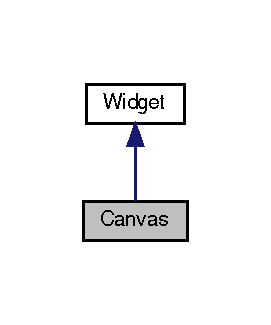
\includegraphics[width=130pt]{classCanvas__inherit__graph}
\end{center}
\end{figure}


Collaboration diagram for Canvas\+:\nopagebreak
\begin{figure}[H]
\begin{center}
\leavevmode
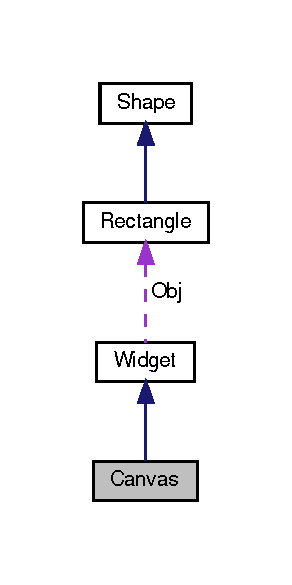
\includegraphics[width=141pt]{classCanvas__coll__graph}
\end{center}
\end{figure}
\subsection*{Additional Inherited Members}


The documentation for this class was generated from the following files\+:\begin{DoxyCompactItemize}
\item 
G\+U\+I.\+h\item 
G\+U\+I.\+cpp\end{DoxyCompactItemize}

\hypertarget{classCanvasClick}{}\doxysection{Canvas\+Click Class Reference}
\label{classCanvasClick}\index{CanvasClick@{CanvasClick}}


Inheritance diagram for Canvas\+Click\+:
\nopagebreak
\begin{figure}[H]
\begin{center}
\leavevmode
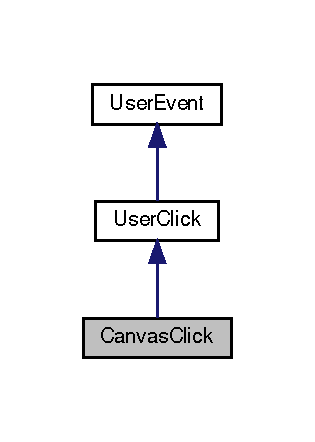
\includegraphics[width=151pt]{classCanvasClick__inherit__graph}
\end{center}
\end{figure}


Collaboration diagram for Canvas\+Click\+:
\nopagebreak
\begin{figure}[H]
\begin{center}
\leavevmode
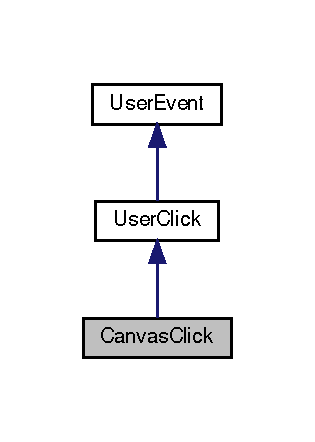
\includegraphics[width=151pt]{classCanvasClick__coll__graph}
\end{center}
\end{figure}
\doxysubsection*{Public Member Functions}
\begin{DoxyCompactItemize}
\item 
\mbox{\Hypertarget{classCanvasClick_aab4d517678c46e8aef85f988dc4785ae}\label{classCanvasClick_aab4d517678c46e8aef85f988dc4785ae}} 
void {\bfseries Generate\+State} (\mbox{\hyperlink{classModel}{Model}} \&m, const std\+::vector$<$ \mbox{\hyperlink{classUserEvent}{User\+Event}} $\ast$ $>$ \&prev\+\_\+events)
\end{DoxyCompactItemize}
\doxysubsection*{Additional Inherited Members}


The documentation for this class was generated from the following file\+:\begin{DoxyCompactItemize}
\item 
Events.\+h\end{DoxyCompactItemize}

\hypertarget{classCanvasInfo}{}\doxysection{Canvas\+Info Class Reference}
\label{classCanvasInfo}\index{CanvasInfo@{CanvasInfo}}


The documentation for this class was generated from the following file\+:\begin{DoxyCompactItemize}
\item 
Model.\+h\end{DoxyCompactItemize}

\hypertarget{classCanvasLayer}{}\doxysection{Canvas\+Layer Class Reference}
\label{classCanvasLayer}\index{CanvasLayer@{CanvasLayer}}


The documentation for this class was generated from the following file\+:\begin{DoxyCompactItemize}
\item 
Model.\+h\end{DoxyCompactItemize}

\hypertarget{classCanvasMouseMove}{}\doxysection{Canvas\+Mouse\+Move Class Reference}
\label{classCanvasMouseMove}\index{CanvasMouseMove@{CanvasMouseMove}}


Inheritance diagram for Canvas\+Mouse\+Move\+:
\nopagebreak
\begin{figure}[H]
\begin{center}
\leavevmode
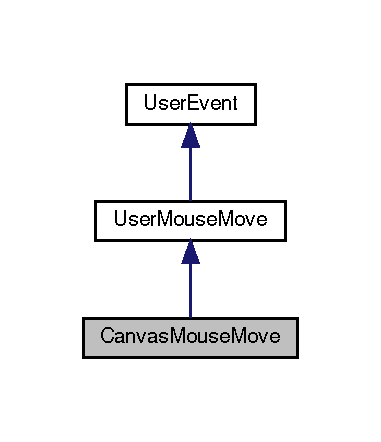
\includegraphics[width=183pt]{classCanvasMouseMove__inherit__graph}
\end{center}
\end{figure}


Collaboration diagram for Canvas\+Mouse\+Move\+:
\nopagebreak
\begin{figure}[H]
\begin{center}
\leavevmode
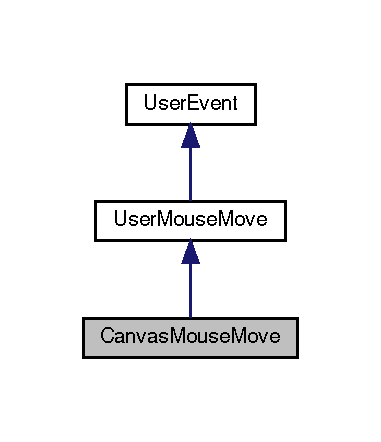
\includegraphics[width=183pt]{classCanvasMouseMove__coll__graph}
\end{center}
\end{figure}
\doxysubsection*{Additional Inherited Members}


The documentation for this class was generated from the following file\+:\begin{DoxyCompactItemize}
\item 
Events.\+h\end{DoxyCompactItemize}

\hypertarget{classController}{}\doxysection{Controller Class Reference}
\label{classController}\index{Controller@{Controller}}
\doxysubsection*{Public Member Functions}
\begin{DoxyCompactItemize}
\item 
\mbox{\Hypertarget{classController_a7dbaa458c5c4a836a697c54fb4d34508}\label{classController_a7dbaa458c5c4a836a697c54fb4d34508}} 
void {\bfseries Finish\+Event\+Sequence} ()
\item 
\mbox{\Hypertarget{classController_a4c94bfb506699fea0583f7c92b084399}\label{classController_a4c94bfb506699fea0583f7c92b084399}} 
bool {\bfseries Manage} (\mbox{\hyperlink{classUserEvent}{User\+Event}} $\ast$e, \mbox{\hyperlink{classModel}{Model}} \&mod, \mbox{\hyperlink{classGUI}{GUI}} \&ui)
\end{DoxyCompactItemize}


The documentation for this class was generated from the following files\+:\begin{DoxyCompactItemize}
\item 
Controller.\+h\item 
Controller.\+cpp\end{DoxyCompactItemize}

\hypertarget{classCreateSquareButton}{}\doxysection{Create\+Square\+Button Class Reference}
\label{classCreateSquareButton}\index{CreateSquareButton@{CreateSquareButton}}


Inheritance diagram for Create\+Square\+Button\+:
\nopagebreak
\begin{figure}[H]
\begin{center}
\leavevmode
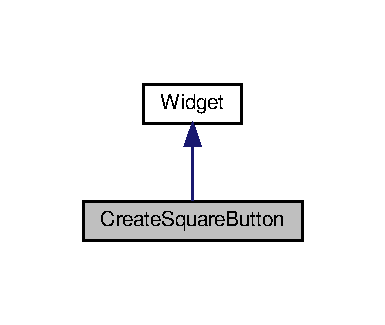
\includegraphics[width=184pt]{classCreateSquareButton__inherit__graph}
\end{center}
\end{figure}


Collaboration diagram for Create\+Square\+Button\+:
\nopagebreak
\begin{figure}[H]
\begin{center}
\leavevmode
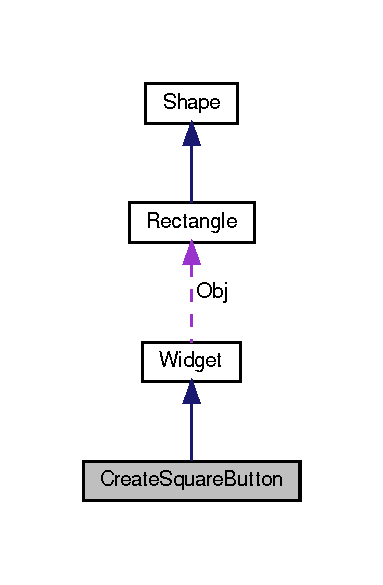
\includegraphics[width=184pt]{classCreateSquareButton__coll__graph}
\end{center}
\end{figure}
\doxysubsection*{Additional Inherited Members}


The documentation for this class was generated from the following file\+:\begin{DoxyCompactItemize}
\item 
GUI.\+h\end{DoxyCompactItemize}

\hypertarget{classCreateTriangleButton}{}\doxysection{Create\+Triangle\+Button Class Reference}
\label{classCreateTriangleButton}\index{CreateTriangleButton@{CreateTriangleButton}}


Inheritance diagram for Create\+Triangle\+Button\+:
\nopagebreak
\begin{figure}[H]
\begin{center}
\leavevmode
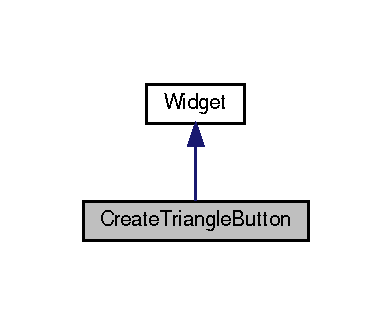
\includegraphics[width=188pt]{classCreateTriangleButton__inherit__graph}
\end{center}
\end{figure}


Collaboration diagram for Create\+Triangle\+Button\+:
\nopagebreak
\begin{figure}[H]
\begin{center}
\leavevmode
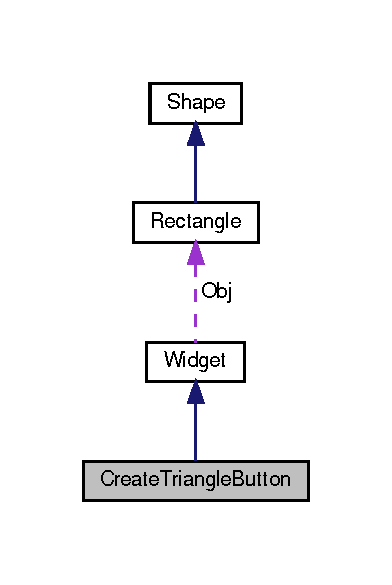
\includegraphics[width=188pt]{classCreateTriangleButton__coll__graph}
\end{center}
\end{figure}
\doxysubsection*{Additional Inherited Members}


The documentation for this class was generated from the following files\+:\begin{DoxyCompactItemize}
\item 
GUI.\+h\item 
GUI.\+cpp\end{DoxyCompactItemize}

\hypertarget{classEmptyEvent}{}\doxysection{Empty\+Event Class Reference}
\label{classEmptyEvent}\index{EmptyEvent@{EmptyEvent}}


Inheritance diagram for Empty\+Event\+:
\nopagebreak
\begin{figure}[H]
\begin{center}
\leavevmode
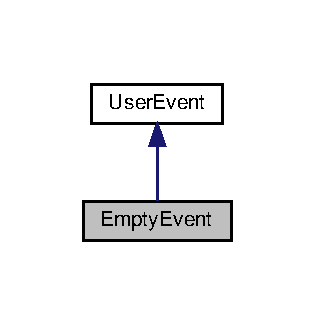
\includegraphics[width=148pt]{classEmptyEvent__inherit__graph}
\end{center}
\end{figure}


Collaboration diagram for Empty\+Event\+:
\nopagebreak
\begin{figure}[H]
\begin{center}
\leavevmode
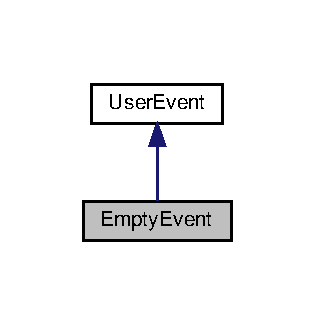
\includegraphics[width=148pt]{classEmptyEvent__coll__graph}
\end{center}
\end{figure}
\doxysubsection*{Additional Inherited Members}


The documentation for this class was generated from the following file\+:\begin{DoxyCompactItemize}
\item 
Events.\+h\end{DoxyCompactItemize}

\hypertarget{classExportButton}{}\section{Export\+Button Class Reference}
\label{classExportButton}\index{Export\+Button@{Export\+Button}}


Inheritance diagram for Export\+Button\+:\nopagebreak
\begin{figure}[H]
\begin{center}
\leavevmode
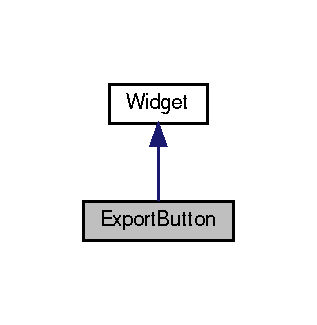
\includegraphics[width=154pt]{classExportButton__inherit__graph}
\end{center}
\end{figure}


Collaboration diagram for Export\+Button\+:\nopagebreak
\begin{figure}[H]
\begin{center}
\leavevmode
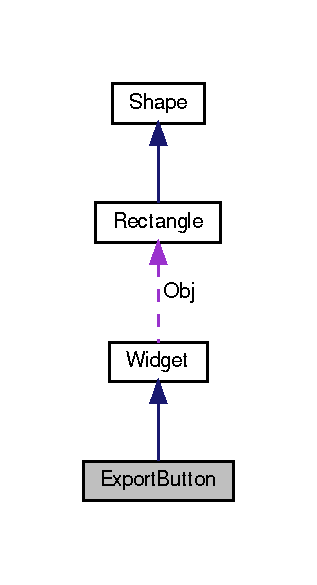
\includegraphics[width=154pt]{classExportButton__coll__graph}
\end{center}
\end{figure}
\subsection*{Public Member Functions}
\begin{DoxyCompactItemize}
\item 
\mbox{\Hypertarget{classExportButton_a76d9c475723745c54a83a1a896bdd900}\label{classExportButton_a76d9c475723745c54a83a1a896bdd900}} 
\hyperlink{classUserEvent}{User\+Event} $\ast$ {\bfseries Click} ()
\end{DoxyCompactItemize}
\subsection*{Additional Inherited Members}


The documentation for this class was generated from the following file\+:\begin{DoxyCompactItemize}
\item 
G\+U\+I.\+h\end{DoxyCompactItemize}

\hypertarget{classGUI}{}\doxysection{GUI Class Reference}
\label{classGUI}\index{GUI@{GUI}}
\doxysubsection*{Public Member Functions}
\begin{DoxyCompactItemize}
\item 
\mbox{\Hypertarget{classGUI_adc6526d47aa2a5715cdea987e6117ef2}\label{classGUI_adc6526d47aa2a5715cdea987e6117ef2}} 
\mbox{\hyperlink{classWidget}{Widget}} $\ast$ {\bfseries Get\+Hovered\+Widget} (\mbox{\hyperlink{structPoint}{Point}} mp)
\item 
\mbox{\Hypertarget{classGUI_ab16d05214befe2474a0b1366a94b068b}\label{classGUI_ab16d05214befe2474a0b1366a94b068b}} 
\mbox{\hyperlink{classUserEvent}{User\+Event}} $\ast$ {\bfseries Hardware\+Event\+Listen} (\mbox{\hyperlink{classHardwareObjects}{Hardware\+Objects}} \&ho)
\end{DoxyCompactItemize}


The documentation for this class was generated from the following files\+:\begin{DoxyCompactItemize}
\item 
GUI.\+h\item 
GUI.\+cpp\end{DoxyCompactItemize}

\hypertarget{classHardwareObjects}{}\section{Hardware\+Objects Class Reference}
\label{classHardwareObjects}\index{Hardware\+Objects@{Hardware\+Objects}}
\subsection*{Public Member Functions}
\begin{DoxyCompactItemize}
\item 
\mbox{\Hypertarget{classHardwareObjects_a8f30f2b7162b5e624d4d9eb0103887b9}\label{classHardwareObjects_a8f30f2b7162b5e624d4d9eb0103887b9}} 
bool {\bfseries Mouse\+Signal} ()
\item 
\mbox{\Hypertarget{classHardwareObjects_a2e08f67779c71674d5117bc54602d86c}\label{classHardwareObjects_a2e08f67779c71674d5117bc54602d86c}} 
bool {\bfseries Mouse\+Click} ()
\item 
\mbox{\Hypertarget{classHardwareObjects_a5483ef1b5b65714249891b12d098e24b}\label{classHardwareObjects_a5483ef1b5b65714249891b12d098e24b}} 
bool {\bfseries Mouse\+Move} ()
\item 
\mbox{\Hypertarget{classHardwareObjects_a901245d20a84651d203fe80b7e6a118f}\label{classHardwareObjects_a901245d20a84651d203fe80b7e6a118f}} 
\hyperlink{structPoint}{Point} {\bfseries Get\+Mouse\+Position} ()
\item 
\mbox{\Hypertarget{classHardwareObjects_a9177dd092805a39d8051cc6895181e31}\label{classHardwareObjects_a9177dd092805a39d8051cc6895181e31}} 
bool {\bfseries Keyboard\+Signal} ()
\item 
\mbox{\Hypertarget{classHardwareObjects_ac18f210a0349fad181f87a513a032047}\label{classHardwareObjects_ac18f210a0349fad181f87a513a032047}} 
char {\bfseries Get\+Clicked\+Key} ()
\item 
\mbox{\Hypertarget{classHardwareObjects_ac9324ff0885a776eacedb2e47b4f26af}\label{classHardwareObjects_ac9324ff0885a776eacedb2e47b4f26af}} 
void {\bfseries Create\+Random\+Event} ()
\item 
\mbox{\Hypertarget{classHardwareObjects_a1b4210606bbaa5a1296f95a738736c1c}\label{classHardwareObjects_a1b4210606bbaa5a1296f95a738736c1c}} 
void {\bfseries Back\+To\+Default} ()
\end{DoxyCompactItemize}


The documentation for this class was generated from the following files\+:\begin{DoxyCompactItemize}
\item 
Hardware\+Objects.\+h\item 
Hardware\+Objects.\+cpp\end{DoxyCompactItemize}

\hypertarget{classImportButton}{}\section{Import\+Button Class Reference}
\label{classImportButton}\index{Import\+Button@{Import\+Button}}


Inheritance diagram for Import\+Button\+:\nopagebreak
\begin{figure}[H]
\begin{center}
\leavevmode
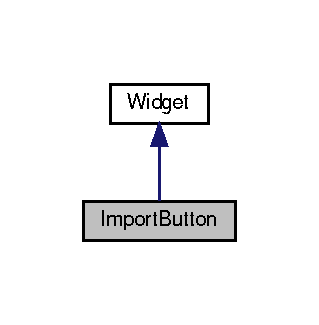
\includegraphics[width=153pt]{classImportButton__inherit__graph}
\end{center}
\end{figure}


Collaboration diagram for Import\+Button\+:\nopagebreak
\begin{figure}[H]
\begin{center}
\leavevmode
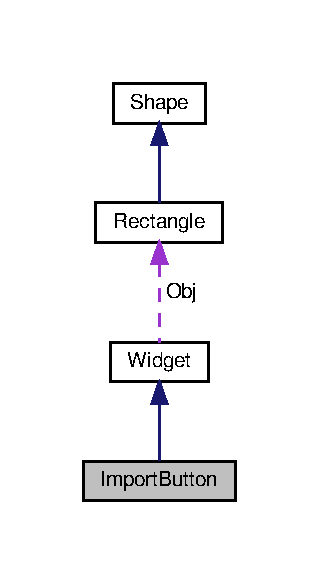
\includegraphics[width=153pt]{classImportButton__coll__graph}
\end{center}
\end{figure}
\subsection*{Public Member Functions}
\begin{DoxyCompactItemize}
\item 
\mbox{\Hypertarget{classImportButton_a2db0b7e9a7fdfc15607f12408f7bb2b4}\label{classImportButton_a2db0b7e9a7fdfc15607f12408f7bb2b4}} 
\hyperlink{classUserEvent}{User\+Event} $\ast$ {\bfseries Click} ()
\end{DoxyCompactItemize}
\subsection*{Additional Inherited Members}


The documentation for this class was generated from the following file\+:\begin{DoxyCompactItemize}
\item 
G\+U\+I.\+h\end{DoxyCompactItemize}

\hypertarget{classKeyboard}{}\doxysection{Keyboard Class Reference}
\label{classKeyboard}\index{Keyboard@{Keyboard}}
\doxysubsection*{Public Member Functions}
\begin{DoxyCompactItemize}
\item 
\mbox{\Hypertarget{classKeyboard_a476c0abf59b76ec5ab44102ee24f38ae}\label{classKeyboard_a476c0abf59b76ec5ab44102ee24f38ae}} 
void {\bfseries Generate\+Random\+Click} ()
\item 
\mbox{\Hypertarget{classKeyboard_aa2c5650fe2599a2418a369c5d9ddab9b}\label{classKeyboard_aa2c5650fe2599a2418a369c5d9ddab9b}} 
void {\bfseries Back\+To\+Default} ()
\item 
\mbox{\Hypertarget{classKeyboard_a0814ccde48eea424e96d0595b3ef2af1}\label{classKeyboard_a0814ccde48eea424e96d0595b3ef2af1}} 
char {\bfseries Get\+Clicked\+Key} ()
\end{DoxyCompactItemize}


The documentation for this class was generated from the following files\+:\begin{DoxyCompactItemize}
\item 
Hardware\+Objects.\+h\item 
Hardware\+Objects.\+cpp\end{DoxyCompactItemize}

\hypertarget{classKeyboardEvent}{}\section{Keyboard\+Event Class Reference}
\label{classKeyboardEvent}\index{Keyboard\+Event@{Keyboard\+Event}}


Inheritance diagram for Keyboard\+Event\+:\nopagebreak
\begin{figure}[H]
\begin{center}
\leavevmode
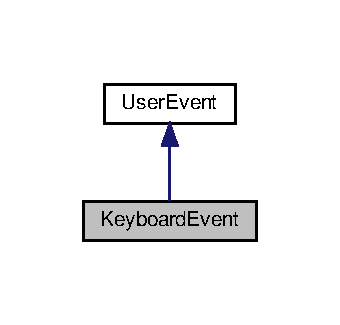
\includegraphics[width=163pt]{classKeyboardEvent__inherit__graph}
\end{center}
\end{figure}


Collaboration diagram for Keyboard\+Event\+:\nopagebreak
\begin{figure}[H]
\begin{center}
\leavevmode
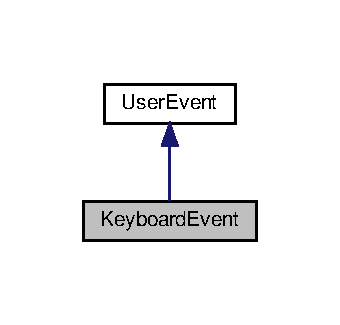
\includegraphics[width=163pt]{classKeyboardEvent__coll__graph}
\end{center}
\end{figure}
\subsection*{Public Member Functions}
\begin{DoxyCompactItemize}
\item 
\mbox{\Hypertarget{classKeyboardEvent_ace85ab376330592de539542e0b190d53}\label{classKeyboardEvent_ace85ab376330592de539542e0b190d53}} 
{\bfseries Keyboard\+Event} (char $\ast$key)
\end{DoxyCompactItemize}
\subsection*{Additional Inherited Members}


The documentation for this class was generated from the following file\+:\begin{DoxyCompactItemize}
\item 
Events.\+h\end{DoxyCompactItemize}

\hypertarget{classKeyboardWidget}{}\doxysection{Keyboard\+Widget Class Reference}
\label{classKeyboardWidget}\index{KeyboardWidget@{KeyboardWidget}}


Inheritance diagram for Keyboard\+Widget\+:
\nopagebreak
\begin{figure}[H]
\begin{center}
\leavevmode
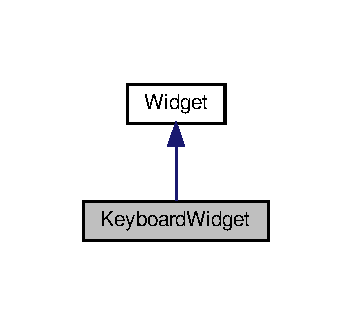
\includegraphics[width=167pt]{classKeyboardWidget__inherit__graph}
\end{center}
\end{figure}


Collaboration diagram for Keyboard\+Widget\+:
\nopagebreak
\begin{figure}[H]
\begin{center}
\leavevmode
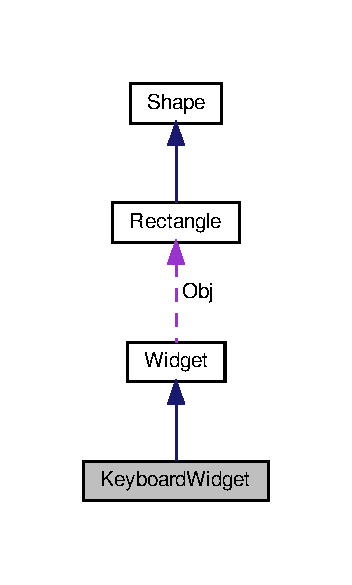
\includegraphics[width=167pt]{classKeyboardWidget__coll__graph}
\end{center}
\end{figure}
\doxysubsection*{Public Member Functions}
\begin{DoxyCompactItemize}
\item 
\mbox{\Hypertarget{classKeyboardWidget_a5d1134565c170b1926256b4712e6acba}\label{classKeyboardWidget_a5d1134565c170b1926256b4712e6acba}} 
\mbox{\hyperlink{classUserEvent}{User\+Event}} $\ast$ {\bfseries Keyboard\+Click} (char c)
\end{DoxyCompactItemize}
\doxysubsection*{Additional Inherited Members}


The documentation for this class was generated from the following files\+:\begin{DoxyCompactItemize}
\item 
GUI.\+h\item 
GUI.\+cpp\end{DoxyCompactItemize}

\hypertarget{classLoadButtonClick}{}\section{Load\+Button\+Click Class Reference}
\label{classLoadButtonClick}\index{Load\+Button\+Click@{Load\+Button\+Click}}


Inheritance diagram for Load\+Button\+Click\+:\nopagebreak
\begin{figure}[H]
\begin{center}
\leavevmode
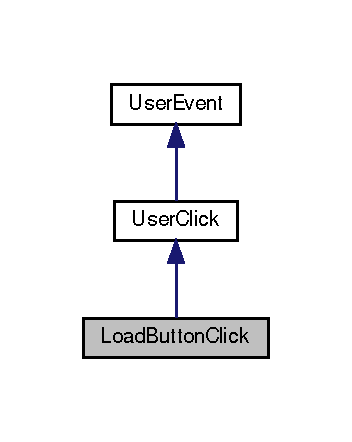
\includegraphics[width=169pt]{classLoadButtonClick__inherit__graph}
\end{center}
\end{figure}


Collaboration diagram for Load\+Button\+Click\+:\nopagebreak
\begin{figure}[H]
\begin{center}
\leavevmode
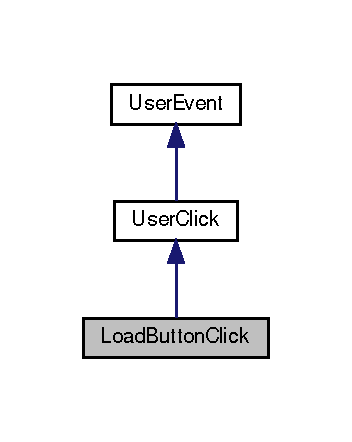
\includegraphics[width=169pt]{classLoadButtonClick__coll__graph}
\end{center}
\end{figure}
\subsection*{Public Member Functions}
\begin{DoxyCompactItemize}
\item 
\mbox{\Hypertarget{classLoadButtonClick_abf958aa98299d099ef1a9e3714e02143}\label{classLoadButtonClick_abf958aa98299d099ef1a9e3714e02143}} 
void {\bfseries Generate\+State} (\hyperlink{classModel}{Model} \&m)
\end{DoxyCompactItemize}
\subsection*{Additional Inherited Members}


The documentation for this class was generated from the following files\+:\begin{DoxyCompactItemize}
\item 
Events.\+h\item 
Events.\+cpp\end{DoxyCompactItemize}

\hypertarget{classModel}{}\section{Model Class Reference}
\label{classModel}\index{Model@{Model}}
\subsection*{Public Member Functions}
\begin{DoxyCompactItemize}
\item 
\mbox{\Hypertarget{classModel_a00377628187a30d8232110df56d15771}\label{classModel_a00377628187a30d8232110df56d15771}} 
void {\bfseries Save\+State\+To\+File} (std\+::string filename)
\item 
\mbox{\Hypertarget{classModel_a64abdebeccd4fcd19d41a14d87aeebd5}\label{classModel_a64abdebeccd4fcd19d41a14d87aeebd5}} 
void {\bfseries Load\+State\+From\+File} (std\+::string filename)
\item 
\mbox{\Hypertarget{classModel_a5842c35a0dda88f6c0bd1e5f8a1ed404}\label{classModel_a5842c35a0dda88f6c0bd1e5f8a1ed404}} 
void {\bfseries Go\+Back\+To\+Previous\+State} ()
\item 
\mbox{\Hypertarget{classModel_a1bc43dc264d3772403975d8e1955ddb0}\label{classModel_a1bc43dc264d3772403975d8e1955ddb0}} 
bool {\bfseries Attach\+State} (\hyperlink{classState}{State} \&s)
\end{DoxyCompactItemize}


The documentation for this class was generated from the following file\+:\begin{DoxyCompactItemize}
\item 
Model.\+h\end{DoxyCompactItemize}

\hypertarget{classMouse}{}\section{Mouse Class Reference}
\label{classMouse}\index{Mouse@{Mouse}}
\subsection*{Public Member Functions}
\begin{DoxyCompactItemize}
\item 
\mbox{\Hypertarget{classMouse_a090db1cdd50702050e51c72bdc2ab322}\label{classMouse_a090db1cdd50702050e51c72bdc2ab322}} 
void {\bfseries Generate\+Random\+Click} ()
\item 
\mbox{\Hypertarget{classMouse_ad909fa9b80d5c9abf6b4f35a4a1ec522}\label{classMouse_ad909fa9b80d5c9abf6b4f35a4a1ec522}} 
void {\bfseries Generate\+Random\+Move} ()
\item 
\mbox{\Hypertarget{classMouse_a3bc5604b4ae13e50d2e1f7b407a052f6}\label{classMouse_a3bc5604b4ae13e50d2e1f7b407a052f6}} 
void {\bfseries Back\+To\+Default} ()
\item 
\mbox{\Hypertarget{classMouse_a6835064c4d4f4ea8e5d85283a8fcca05}\label{classMouse_a6835064c4d4f4ea8e5d85283a8fcca05}} 
\hyperlink{structPoint}{Point} {\bfseries Get\+Mouse\+Pos} ()
\end{DoxyCompactItemize}


The documentation for this class was generated from the following files\+:\begin{DoxyCompactItemize}
\item 
Hardware\+Objects.\+h\item 
Hardware\+Objects.\+cpp\end{DoxyCompactItemize}

\hypertarget{structPoint}{}\section{Point Struct Reference}
\label{structPoint}\index{Point@{Point}}
\subsection*{Public Attributes}
\begin{DoxyCompactItemize}
\item 
\mbox{\Hypertarget{structPoint_a8c779e11e694b20e0946105a9f5de842}\label{structPoint_a8c779e11e694b20e0946105a9f5de842}} 
int {\bfseries x}
\item 
\mbox{\Hypertarget{structPoint_a2e1b5fb2b2a83571f5c0bc0f66a73cf7}\label{structPoint_a2e1b5fb2b2a83571f5c0bc0f66a73cf7}} 
int {\bfseries y}
\item 
\mbox{\Hypertarget{structPoint_a5eec80a5eba17a6cfc509a17125a5f17}\label{structPoint_a5eec80a5eba17a6cfc509a17125a5f17}} 
int {\bfseries r}
\item 
\mbox{\Hypertarget{structPoint_a9e9b4b8434c0d9ca60c34a98a57d341b}\label{structPoint_a9e9b4b8434c0d9ca60c34a98a57d341b}} 
int {\bfseries g}
\item 
\mbox{\Hypertarget{structPoint_ade275c6d86d695a9b4d8f7affaef4719}\label{structPoint_ade275c6d86d695a9b4d8f7affaef4719}} 
int {\bfseries b}
\item 
\mbox{\Hypertarget{structPoint_a6c521917e69db0f084cc3ea925d54c1c}\label{structPoint_a6c521917e69db0f084cc3ea925d54c1c}} 
double {\bfseries opacity}
\end{DoxyCompactItemize}


The documentation for this struct was generated from the following file\+:\begin{DoxyCompactItemize}
\item 
Primitives.\+h\end{DoxyCompactItemize}

\hypertarget{structRectangle}{}\section{Rectangle Struct Reference}
\label{structRectangle}\index{Rectangle@{Rectangle}}


Inheritance diagram for Rectangle\+:\nopagebreak
\begin{figure}[H]
\begin{center}
\leavevmode
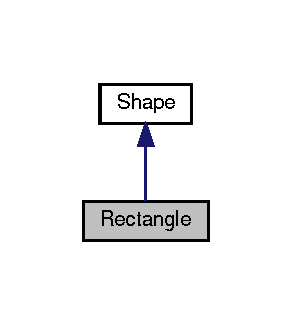
\includegraphics[width=141pt]{structRectangle__inherit__graph}
\end{center}
\end{figure}


Collaboration diagram for Rectangle\+:\nopagebreak
\begin{figure}[H]
\begin{center}
\leavevmode
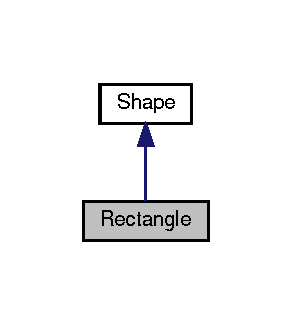
\includegraphics[width=141pt]{structRectangle__coll__graph}
\end{center}
\end{figure}
\subsection*{Public Member Functions}
\begin{DoxyCompactItemize}
\item 
\mbox{\Hypertarget{structRectangle_afda3a0efab405eb647361ad1edbd0e95}\label{structRectangle_afda3a0efab405eb647361ad1edbd0e95}} 
void {\bfseries Set\+Shape\+Dimensions} ()
\item 
\mbox{\Hypertarget{structRectangle_a0ea219073799a22f59de30421792e86b}\label{structRectangle_a0ea219073799a22f59de30421792e86b}} 
bool {\bfseries Contains} (\hyperlink{structPoint}{Point} p)
\item 
\mbox{\Hypertarget{structRectangle_addb2bfa9829eaa920bebdcf0bebe9bc9}\label{structRectangle_addb2bfa9829eaa920bebdcf0bebe9bc9}} 
{\bfseries Rectangle} (int xl=0, int yl=0, int xr=0, int yr=0)
\end{DoxyCompactItemize}
\subsection*{Public Attributes}
\begin{DoxyCompactItemize}
\item 
\mbox{\Hypertarget{structRectangle_aab16fa89eb9ab46d69dd6cefcb367a13}\label{structRectangle_aab16fa89eb9ab46d69dd6cefcb367a13}} 
std\+::vector$<$ \hyperlink{structPoint}{Point} $\ast$ $>$ {\bfseries m\+Corner\+Points}
\item 
\mbox{\Hypertarget{structRectangle_a87c944bf4e21793fa46ca5a06c2e09f8}\label{structRectangle_a87c944bf4e21793fa46ca5a06c2e09f8}} 
int {\bfseries m\+Xl}
\item 
\mbox{\Hypertarget{structRectangle_a187ffc864e8d9799077cd74052bda9d5}\label{structRectangle_a187ffc864e8d9799077cd74052bda9d5}} 
int {\bfseries m\+Yl}
\item 
\mbox{\Hypertarget{structRectangle_ac00e1c51a17a533ac2e82c6a80ef4405}\label{structRectangle_ac00e1c51a17a533ac2e82c6a80ef4405}} 
int {\bfseries m\+Xr}
\item 
\mbox{\Hypertarget{structRectangle_a044a4c391bfa2eaf81a546387fee9125}\label{structRectangle_a044a4c391bfa2eaf81a546387fee9125}} 
int {\bfseries m\+Yr}
\end{DoxyCompactItemize}


The documentation for this struct was generated from the following file\+:\begin{DoxyCompactItemize}
\item 
Primitives.\+h\end{DoxyCompactItemize}

\hypertarget{classSaveButton}{}\doxysection{Save\+Button Class Reference}
\label{classSaveButton}\index{SaveButton@{SaveButton}}


Inheritance diagram for Save\+Button\+:
\nopagebreak
\begin{figure}[H]
\begin{center}
\leavevmode
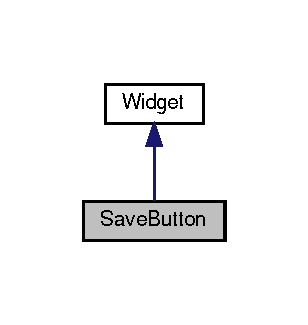
\includegraphics[width=148pt]{classSaveButton__inherit__graph}
\end{center}
\end{figure}


Collaboration diagram for Save\+Button\+:
\nopagebreak
\begin{figure}[H]
\begin{center}
\leavevmode
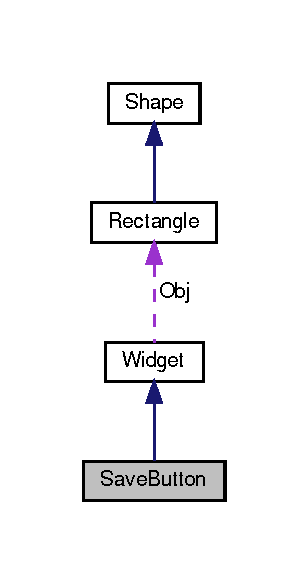
\includegraphics[width=148pt]{classSaveButton__coll__graph}
\end{center}
\end{figure}
\doxysubsection*{Public Member Functions}
\begin{DoxyCompactItemize}
\item 
\mbox{\Hypertarget{classSaveButton_af5a177a907bced69df780571328ee073}\label{classSaveButton_af5a177a907bced69df780571328ee073}} 
\mbox{\hyperlink{classUserEvent}{User\+Event}} $\ast$ {\bfseries Click} ()
\end{DoxyCompactItemize}
\doxysubsection*{Additional Inherited Members}


The documentation for this class was generated from the following files\+:\begin{DoxyCompactItemize}
\item 
GUI.\+h\item 
GUI.\+cpp\end{DoxyCompactItemize}

\hypertarget{classSaveButtonClick}{}\section{Save\+Button\+Click Class Reference}
\label{classSaveButtonClick}\index{Save\+Button\+Click@{Save\+Button\+Click}}


Inheritance diagram for Save\+Button\+Click\+:\nopagebreak
\begin{figure}[H]
\begin{center}
\leavevmode
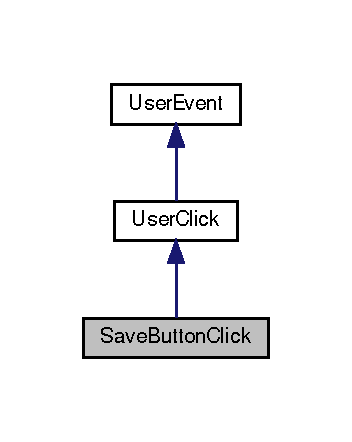
\includegraphics[width=170pt]{classSaveButtonClick__inherit__graph}
\end{center}
\end{figure}


Collaboration diagram for Save\+Button\+Click\+:\nopagebreak
\begin{figure}[H]
\begin{center}
\leavevmode
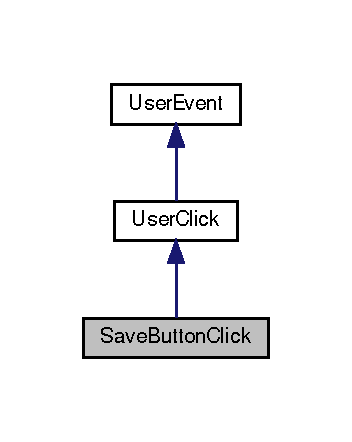
\includegraphics[width=170pt]{classSaveButtonClick__coll__graph}
\end{center}
\end{figure}
\subsection*{Public Member Functions}
\begin{DoxyCompactItemize}
\item 
\mbox{\Hypertarget{classSaveButtonClick_af54ca18155e6a8f40e55d80a825cdd8e}\label{classSaveButtonClick_af54ca18155e6a8f40e55d80a825cdd8e}} 
void {\bfseries Generate\+State} (\hyperlink{classModel}{Model} \&m)
\item 
\mbox{\Hypertarget{classSaveButtonClick_a0db27b6afd24cd8533c916159d20f758}\label{classSaveButtonClick_a0db27b6afd24cd8533c916159d20f758}} 
void {\bfseries Generate\+State} (\hyperlink{classModel}{Model} \&m, const std\+::vector$<$ \hyperlink{classUserEvent}{User\+Event} $\ast$$>$ \&prev\+\_\+events)
\item 
\mbox{\Hypertarget{classSaveButtonClick_a0317281e7e59a36f12c88699cab36572}\label{classSaveButtonClick_a0317281e7e59a36f12c88699cab36572}} 
void {\bfseries Update\+View} (\hyperlink{classGUI}{G\+UI} \&ui)
\end{DoxyCompactItemize}
\subsection*{Additional Inherited Members}


The documentation for this class was generated from the following files\+:\begin{DoxyCompactItemize}
\item 
Events.\+h\item 
Events.\+cpp\end{DoxyCompactItemize}

\hypertarget{structShape}{}\section{Shape Struct Reference}
\label{structShape}\index{Shape@{Shape}}


Inheritance diagram for Shape\+:\nopagebreak
\begin{figure}[H]
\begin{center}
\leavevmode
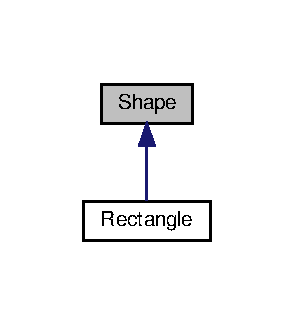
\includegraphics[width=141pt]{structShape__inherit__graph}
\end{center}
\end{figure}
\subsection*{Public Attributes}
\begin{DoxyCompactItemize}
\item 
\mbox{\Hypertarget{structShape_a5a45763b84f2bd7b7cd6bf58841b612c}\label{structShape_a5a45763b84f2bd7b7cd6bf58841b612c}} 
bool {\bfseries m\+Is\+Complete}
\item 
\mbox{\Hypertarget{structShape_a86bf2e7e1c578665974a725dfabf6f5b}\label{structShape_a86bf2e7e1c578665974a725dfabf6f5b}} 
std\+::vector$<$ \hyperlink{structPoint}{Point} $\ast$ $>$ {\bfseries m\+Points}
\end{DoxyCompactItemize}


The documentation for this struct was generated from the following file\+:\begin{DoxyCompactItemize}
\item 
Primitives.\+h\end{DoxyCompactItemize}

\hypertarget{classState}{}\section{State Class Reference}
\label{classState}\index{State@{State}}


The documentation for this class was generated from the following file\+:\begin{DoxyCompactItemize}
\item 
Model.\+h\end{DoxyCompactItemize}

\hypertarget{classUserClick}{}\doxysection{User\+Click Class Reference}
\label{classUserClick}\index{UserClick@{UserClick}}


Inheritance diagram for User\+Click\+:
\nopagebreak
\begin{figure}[H]
\begin{center}
\leavevmode
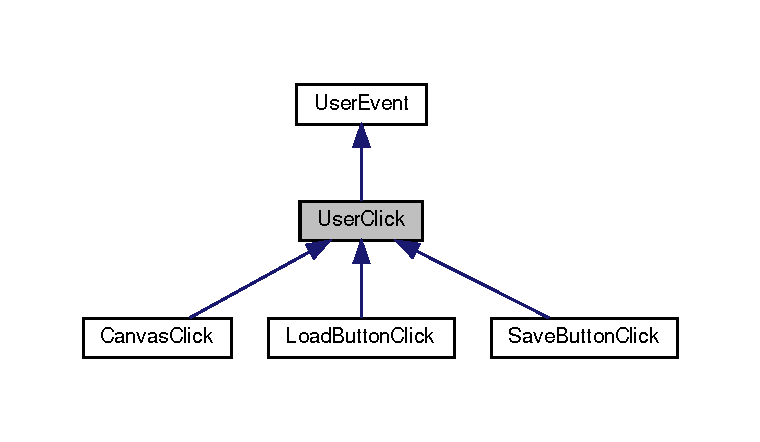
\includegraphics[width=350pt]{classUserClick__inherit__graph}
\end{center}
\end{figure}


Collaboration diagram for User\+Click\+:
\nopagebreak
\begin{figure}[H]
\begin{center}
\leavevmode
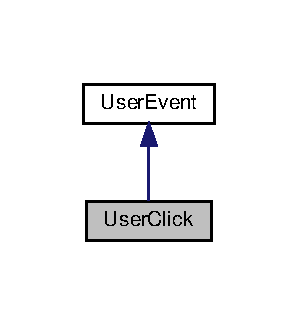
\includegraphics[width=142pt]{classUserClick__coll__graph}
\end{center}
\end{figure}
\doxysubsection*{Additional Inherited Members}


The documentation for this class was generated from the following file\+:\begin{DoxyCompactItemize}
\item 
Events.\+h\end{DoxyCompactItemize}

\hypertarget{classUserEvent}{}\section{User\+Event Class Reference}
\label{classUserEvent}\index{User\+Event@{User\+Event}}


Inheritance diagram for User\+Event\+:\nopagebreak
\begin{figure}[H]
\begin{center}
\leavevmode
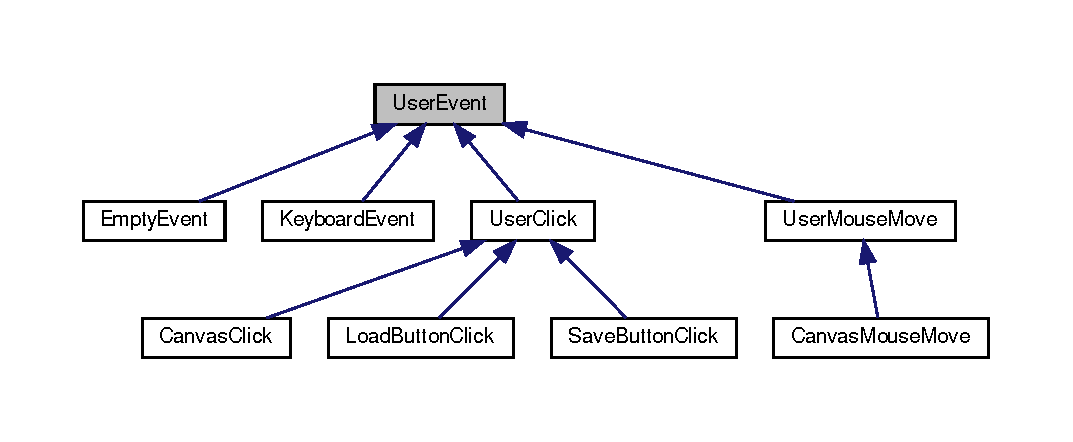
\includegraphics[width=350pt]{classUserEvent__inherit__graph}
\end{center}
\end{figure}
\subsection*{Public Member Functions}
\begin{DoxyCompactItemize}
\item 
\mbox{\Hypertarget{classUserEvent_ad2c66a7c1dbf277ad147fd4336f5f60a}\label{classUserEvent_ad2c66a7c1dbf277ad147fd4336f5f60a}} 
std\+::string {\bfseries Get\+Type} ()
\item 
\mbox{\Hypertarget{classUserEvent_a9e8a9f0fd1f200fbd099d02dae3792cb}\label{classUserEvent_a9e8a9f0fd1f200fbd099d02dae3792cb}} 
void {\bfseries Generate\+State} (\hyperlink{classModel}{Model} \&m)
\item 
\mbox{\Hypertarget{classUserEvent_a196963d228e1cdd314043dfa3bdc8f2d}\label{classUserEvent_a196963d228e1cdd314043dfa3bdc8f2d}} 
void {\bfseries Generate\+State} (\hyperlink{classModel}{Model} \&m, const std\+::vector$<$ \hyperlink{classUserEvent}{User\+Event} $\ast$$>$ \&prev\+\_\+events)
\item 
\mbox{\Hypertarget{classUserEvent_ae844d6d647e6dd6bcc6d81b3f959782e}\label{classUserEvent_ae844d6d647e6dd6bcc6d81b3f959782e}} 
void {\bfseries Update\+View} (\hyperlink{classGUI}{G\+UI} \&ui)
\item 
\mbox{\Hypertarget{classUserEvent_a394a8268528c11de6b3e358d578f8d78}\label{classUserEvent_a394a8268528c11de6b3e358d578f8d78}} 
bool {\bfseries Expect\+Smth} ()
\item 
\mbox{\Hypertarget{classUserEvent_a1e0c7ec71a63e51bd2f231c3a9cccf50}\label{classUserEvent_a1e0c7ec71a63e51bd2f231c3a9cccf50}} 
bool {\bfseries Expect} (\hyperlink{classUserEvent}{User\+Event} $\ast$prev)
\end{DoxyCompactItemize}
\subsection*{Protected Attributes}
\begin{DoxyCompactItemize}
\item 
\mbox{\Hypertarget{classUserEvent_a587f493f4e1179b28114d6b001857569}\label{classUserEvent_a587f493f4e1179b28114d6b001857569}} 
std\+::string {\bfseries m\+Type}
\item 
\mbox{\Hypertarget{classUserEvent_a854dd5059f7c0f9edb7a59721cedd5a2}\label{classUserEvent_a854dd5059f7c0f9edb7a59721cedd5a2}} 
std\+::set$<$ std\+::string $>$ {\bfseries m\+Possible\+Correct\+Next\+Events} = \{\}
\end{DoxyCompactItemize}


The documentation for this class was generated from the following files\+:\begin{DoxyCompactItemize}
\item 
Events.\+h\item 
Events.\+cpp\end{DoxyCompactItemize}

\hypertarget{classUserInfo}{}\section{User\+Info Class Reference}
\label{classUserInfo}\index{User\+Info@{User\+Info}}


The documentation for this class was generated from the following file\+:\begin{DoxyCompactItemize}
\item 
Model.\+h\end{DoxyCompactItemize}

\hypertarget{classUserMouseMove}{}\doxysection{User\+Mouse\+Move Class Reference}
\label{classUserMouseMove}\index{UserMouseMove@{UserMouseMove}}


Inheritance diagram for User\+Mouse\+Move\+:
\nopagebreak
\begin{figure}[H]
\begin{center}
\leavevmode
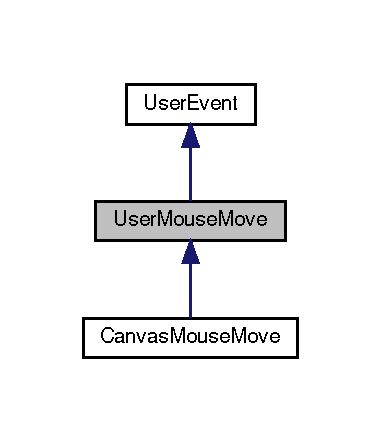
\includegraphics[width=183pt]{classUserMouseMove__inherit__graph}
\end{center}
\end{figure}


Collaboration diagram for User\+Mouse\+Move\+:
\nopagebreak
\begin{figure}[H]
\begin{center}
\leavevmode
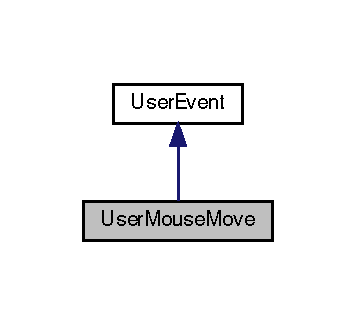
\includegraphics[width=171pt]{classUserMouseMove__coll__graph}
\end{center}
\end{figure}
\doxysubsection*{Additional Inherited Members}


The documentation for this class was generated from the following file\+:\begin{DoxyCompactItemize}
\item 
Events.\+h\end{DoxyCompactItemize}

\hypertarget{classWidget}{}\doxysection{Widget Class Reference}
\label{classWidget}\index{Widget@{Widget}}


Inheritance diagram for Widget\+:
\nopagebreak
\begin{figure}[H]
\begin{center}
\leavevmode
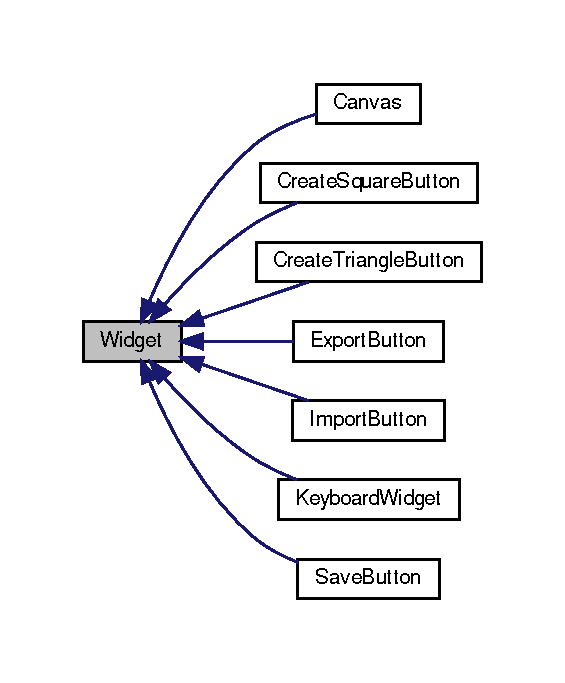
\includegraphics[width=271pt]{classWidget__inherit__graph}
\end{center}
\end{figure}


Collaboration diagram for Widget\+:
\nopagebreak
\begin{figure}[H]
\begin{center}
\leavevmode
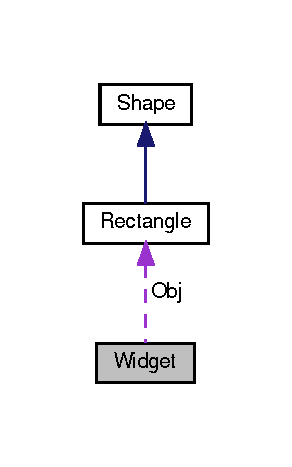
\includegraphics[width=140pt]{classWidget__coll__graph}
\end{center}
\end{figure}
\doxysubsection*{Public Member Functions}
\begin{DoxyCompactItemize}
\item 
\mbox{\Hypertarget{classWidget_add4af843fbd014c334c40216cd440913}\label{classWidget_add4af843fbd014c334c40216cd440913}} 
bool {\bfseries Check\+If\+Hovered} (\mbox{\hyperlink{structPoint}{Point}} P)
\item 
\mbox{\Hypertarget{classWidget_a617f4ee017d17bcae89a33ffb5affde6}\label{classWidget_a617f4ee017d17bcae89a33ffb5affde6}} 
\mbox{\hyperlink{classUserEvent}{User\+Event}} $\ast$ {\bfseries Click} ()
\item 
\mbox{\Hypertarget{classWidget_ad583f576b84f40227987b38c1b5da5bd}\label{classWidget_ad583f576b84f40227987b38c1b5da5bd}} 
\mbox{\hyperlink{classUserEvent}{User\+Event}} $\ast$ {\bfseries Hover} ()
\end{DoxyCompactItemize}
\doxysubsection*{Protected Attributes}
\begin{DoxyCompactItemize}
\item 
\mbox{\Hypertarget{classWidget_a877ee32cf2532d36696a74e4b2e8a08d}\label{classWidget_a877ee32cf2532d36696a74e4b2e8a08d}} 
\mbox{\hyperlink{structRectangle}{Rectangle}} {\bfseries Obj}
\end{DoxyCompactItemize}


The documentation for this class was generated from the following files\+:\begin{DoxyCompactItemize}
\item 
GUI.\+h\item 
GUI.\+cpp\end{DoxyCompactItemize}

%--- End generated contents ---

% Index
\backmatter
\newpage
\phantomsection
\clearemptydoublepage
\addcontentsline{toc}{chapter}{Index}
\printindex

\end{document}
